\documentclass[]{beamer}

\usepackage[T1]{fontenc}
\usepackage[english]{babel}
%\usepackage[utf8]{inputenc}
\usepackage[babel]{csquotes}
\usepackage{graphicx}
\usepackage{lmodern}
\usepackage{textcomp}
\usepackage{booktabs}
%\usepackage{caption}
\usepackage{tipa}
\usepackage{gb4e}
\noautomath
\usepackage{subfigure}

\setbeamertemplate{section in toc}[sections numbered]

\setbeamercovered{transparent}
\setbeamertemplate{footline}[frame number]

\usepackage[backend=biber, 
					style=authoryear-comp, %ebd. %keine ebd.: comp, kompakt
						dashed=false,
						sorting=nyt,	%Name, Year, Title
						maxbibnames=13,
						minbibnames=13, % in der Bibliography Anzahl der Namen in Listen
						maxcitenames=2,
						mincitenames=1, % in der Zitation Anzahl der Namen
						isbn=false,
						url=true,
						doi=false,
						eprint=false,
						block=space % horzontaler Platz zw. Feldern
						]{biblatex}



\addbibresource{literature.bib}
\bibliography{literature}
\renewcommand{\bibfont}{\tiny}

%\titlegraphic{}
\title[]{COST Action Distant Reading for European Literary History}
\subtitle[]{Corpus design and text contribution for ELTeC \\ 

\includegraphics[scale=0.35]{pics/distantreadinglogo-high-300x138.png}
}
\date[]{\small \textcolor[rgb]{0.4,0.4,0.4}{TS Distant Reading for European Literary History, Budapest, 09/23-09/25 2019}}
\author[]{\textcolor[rgb]{0,0,0}{Lou Burnard, Carolin Odebrecht, Christian Reul and Martina Scholger}}
%\institute[]{\textcolor[rgb]{0,0,0}{}}

\begin{document}

%\setcounter{framenumber}{-1}
\frame{
  \titlepage
}

\frame{
\frametitle{Introduction}

\begin{itemize}
	\item metadata for novels in ELTeC
	\item introduction to metadata schema
	\item metadata collection with world cat
	\item encoding metadata in TEI schema
\end{itemize}
}


\begin{frame}
	\frametitle{Outline}
	\tableofcontents
\end{frame}

\section{WG Scholary Resources and ELTeC}

\begin{frame}
	\frametitle{Outline}
	\tableofcontents[currentsection]
\end{frame}

\frame{
\frametitle{Working Group 1: \textsc{Scholarly Resources}}
\begin{itemize}
	\item Creating an open source multi-lingual benchmark corpus for European literature of the 19th century (novels):
	European Literary Text Collection (ELTeC)\footnote{\url{https://www.distant-reading.net/wg-1/}}
	\item 34 Members from 22 countries
	\item Main tasks are
	\begin{itemize}
		\item defining corpus design
		\item developing basic encoding schemas
		\item developing workflows
	\end{itemize}
\end{itemize}
}

\frame{
\frametitle{Corpus design}

Corpus design defines two things \parencites[cf.][]{LudelingRitzStedeEtAl2016,Hunston2008}:
	\begin{itemize}
		\item candidates $\rightarrow$ sampling
		\begin{itemize}
			\item Which text(s) can be included in the corpus? Which can't?
		\end{itemize}
		\item proportion $\rightarrow$ balancing
		\begin{itemize}
			\item How many texts with which characteristics should the corpus contain? 
		\end{itemize}
	\end{itemize}
}

\frame{
\frametitle{Corpus design -- approach of WG1}

\begin{itemize}
\item Sampling and balancing criteria\footnote{\tiny\url{https://github.com/distantreading/WG1/blob/master/sampling_proposal.xml}} will
\begin{itemize}
	\item not define what a novel is (cf. WG 3)
	\item follow a non-normative but metadata-based approach (not canon-based)\footnote{Each canon is
                    a result of rating texts from different perspectives: intellectual, economical, or/and reader rating \parencites[a.o.][]{Winko1996,Herrmann2011}.}
	\item aim to represent the variety of a population\footnote{Cf. for discussion of representativeness \textcite{Biber1993} and canonicity and corpus design \textcites{AlgeeHewittMcGurl2018,BodeKatherine2018AWoF}.}
	\item allow for a comparability of texts and individual sub-collections according to different metadata set(s)
\end{itemize}
\end{itemize}
}

\frame{
\frametitle{Sampling criteria}

\begin{itemize}
	\item \textbf{language}: European languages, no translations
	\item \textbf{prose}: narrative fictional prose
	\item \textbf{period}: 1840--1920
	\item \textbf{length}: min. 10.000 words
		\item \textbf{publication}: prefer books over novels published in serial publications
	\item \textbf{access}: only freely available digitizations
\end{itemize}

}
\frame{
\frametitle{Balancing criteria}

100 texts per language (language collection)
	\begin{itemize}
		\item \textbf{period}: distribution over time
		\begin{itemize}
			\item group T1: 1840-1859
			\item group T2: 1860-1879
			\item group T3: 1880-1899
			\item group T4: 1900-1920
		\end{itemize}
		\item \textbf{gender}: min. 10\% and max. 50\% written by female authors
		\item \textbf{authorship}: 9 - 11 authors with exactly three novels (otherwise, only one text for each author)
		\item \textbf{length}: min. 20\% are short novels (10-50k word tokens), min. 20\% are long novels (>100k word tokens).
		\item \textbf{reprint}: min. 30\% are highly canonized novels, min. 30\% should be non-canonized novels, based reprint counts within the period 1970-2009 (work in progress)
	\end{itemize}
}

\frame{
\frametitle{(ideal) Composition}

\begin{figure}%
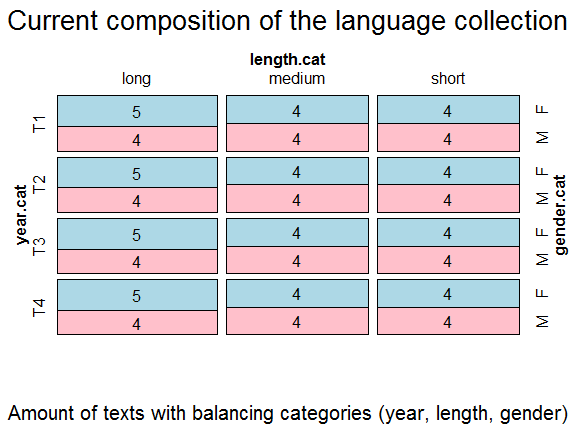
\includegraphics[scale=0.5]{pics/Rplot-balanced.png}%
\end{figure}

}

\frame{
\frametitle{Example: German Text Collection}

\begin{figure}%
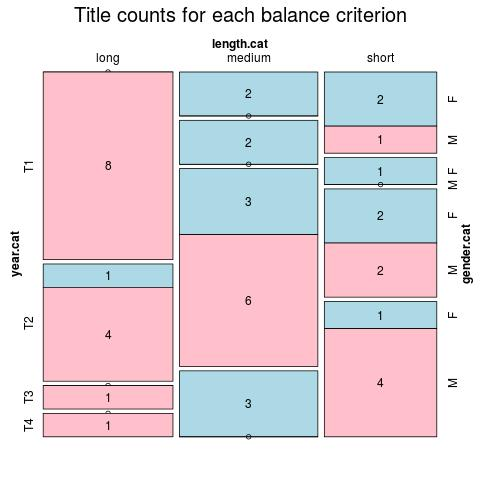
\includegraphics[scale=0.4]{pics/mosaic.png}%

\end{figure}

}

\section{ELTeC Encoding Schema -- Metadata}
\begin{frame}
	\frametitle{Outline}
	\tableofcontents[currentsection]
\end{frame}

\frame{
\frametitle{TEI encoding for ELTeC}

Sources:
\begin{itemize}
	\item different texts levels / editions \parencite[cf. e.g.][]{IFLA2009}
	\item different levels of digitization/annotation
	\item various languages, encodings, fonts
	\end{itemize} \pause
	
Corpus:
	\begin{itemize}
	\item minimal, uniform encoding (applicable for different sources)
	\item text representation focus on consistency and simplicity (not full complexity/richness needed for digital editions)
	\item basic metadata and references (not replicating work of libraries)
	\item serves as master file container for automatically generating transformations, annotations and derivations
\end{itemize}
}

\frame{
\frametitle{Encoding levels for ELTeC}

TEI ODD-chain\footnote{Cf. TEI ODD \textcite{BurnardRahtz2004}, for documentation of ELTeC ODD \url{https://github.com/distantreading/WG1}} provides different levels of encoding:
	\begin{itemize}
		\item \textbf{level0}: basic encoding with e.g. paragraph, heading, page break, text division, 
		\item \textbf{level1}: richer encoding, adding e.g. font change, graphic, quotation, correction
		\item \textbf{level2}: token-based encoding with automatic lemmatization and part-of-speech annotation
		\item[$\rightarrow$] consistent metadata for each level of encoding
	\end{itemize}
}

\frame{
\frametitle{Metadata schema}

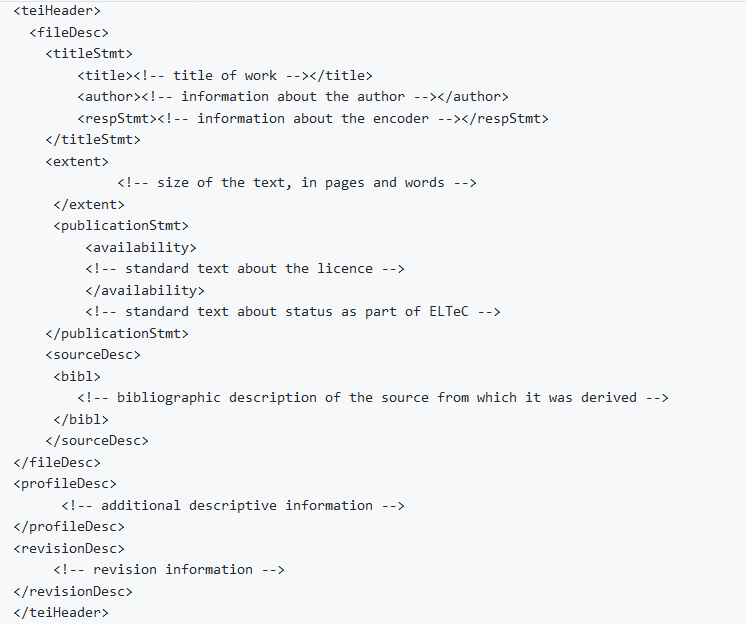
\includegraphics[scale=0.5]{pics/header.png}

}

\frame{
\frametitle{TEI document, encoding level 1}

\begin{figure}[htb]
        \centering
        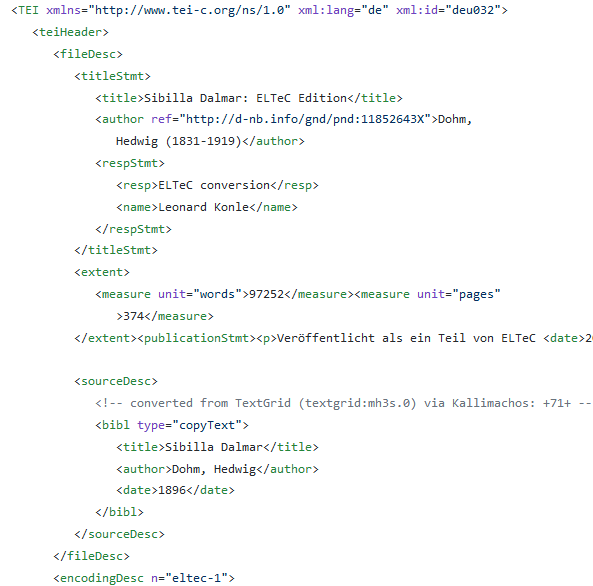
\includegraphics[scale=0.5]{pics/dohm2.png}\footnote{\tiny \url{https://github.com/COST-ELTeC/ELTeC-deu/blob/master/level1/deu032.xml}}
\end{figure}
}

\section{Research for metadata -- World cat}
\begin{frame}
	\frametitle{Outline}
	\tableofcontents[currentsection]
\end{frame}

\frame{
\frametitle{Research for metadata}

\begin{itemize}
	\item Using \textit{worldcat} to get required metadata
	\item \url{https://www.worldcat.org/}
\end{itemize}

}

\frame[allowframebreaks]{
\frametitle{References}
\printbibliography
}

\end{document}


%%%%%%%%%%%% Slides introduction to COST and WG1 %%%%%%%%%%%%%%%%
%\section{COST Action}
%
%\frame{
%\frametitle{COST}
%
%\begin{itemize}
	%\item European Cooperation in Science and Technology = COST\footnote{\url{www.cost.eu}}
		%\item EU funding since 1971
		%\item COST Actions are research networks
		%\begin{itemize}
				%\item for any scientific field,
				%\item for workshops, conferences, working group meetings, training schools, short-term scientific missions, and dissemination and communication activities,
				%\item for fostering Inclusiveness Target Countries (ITC).
		%\end{itemize}
		%\item Each country member has a national supporting institution\footnote{For Germany it's BMBF \url{https://www.cost.dlr.de/}}
%\end{itemize}
%}
%
%\frame{
%\frametitle{COST Action}
%
%\begin{itemize}
	%\item Application for funding:
	%\begin{itemize}
		%\item Submission of a proposal with min. 7 COST Members\footnote{With 50 \% ITC, member countries: \url{https://www.cost.eu/who-we-are/members/}}
		%\item Project programme lasting four years
		%\item Funding for networking tools (meetings, training schools, workshops etc.)
	%\end{itemize}\pause
		%\item Organisation of the Action:
		%\begin{itemize}
			%\item Management Committee: each country is represented by regular and substitute members (planing, votes on budget plans, activities etc.)
			%\item Core Group: Coordinating roles (tasks, milestones, activities)
			%\item Working Groups
			%\item Science Officer and Administrative Officer 
		%\end{itemize}
%\end{itemize}
%}
%
%\frame{
%\frametitle{COST Action Distant Reading}
%
%\begin{itemize}
	%\item Christof Sch\"och, University of Trier
	%\item CA16204 will
	%\begin{itemize}
		%\item \glqq{}create a vibrant and diverse network of researchers jointly developing the resources and methods necessary to change the way European literary history is written\grqq{}
		%\item \glqq{}contribute to the development and distribution of methods, competencies, data, best practices, standards and tools relevant to Distant Reading research\grqq{}\footnote{\url{www.distant-reading.net}}
		%\item started autumn 2017
	%\end{itemize}
	%\item Working groups
	%\begin{itemize}
		%\item WG 1: Scholarly Resources
		%\item WG 2: Methods and Tools
		%\item WG 3: Literary Theory and History
		%\item WG 4: Dissemination
	%\end{itemize}
%\end{itemize}
%}
%
%\frame{
%\frametitle{COST Action Distant Reading}
%\begin{figure}%
%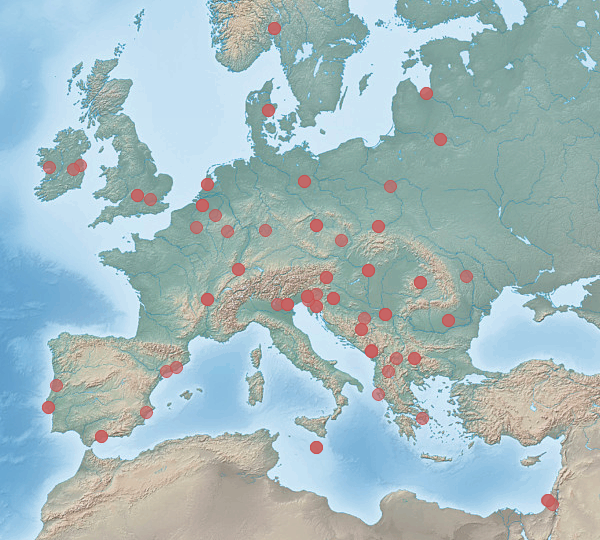
\includegraphics[scale=.4]{pics/map.png}\footnote{\url{https://www.distant-reading.net/about/network/}}%
%\end{figure}
%}

